\newpage
\section{Triangles on a Cone}	


\begin{prob}
Put a dot at the center of a blank sheet of paper and call it $\vec{o}$.
Use a protractor to draw an angle of $50^\circ$ with vertex at the
point $\vec{o}$ and sides extending all the way out to the edge of the
paper.  Cut the paper along one side of the angle and one side only.
Make a cone by moving the cut edge to the other side of the angle you
drew.  This cone (extended infinitely) is your universe.
\end{prob}


\begin{prob}
Make a triangle in your universe that surrounds $\vec{o}$. To do this,
unfold your universe and lay it out flat on the desk and make the
sides with your ruler.  When a side gets to the cut side of your
angle, put the other side of the angle on top and keep going.
\end{prob}

\begin{prob}
You measure angles on your universe by laying the paper out flat and
measuring the angles on the paper. Measure the angles in your
triangle, what do they sum to?
\end{prob}


\begin{prob}
Repeat the problems above, but this time cut an angle of $40^\circ$ to
make your cone. What do you notice?
\end{prob}

Let's see if we can explain this. Do you know who is eager to help
you? That's right: Louie Llama.
\[
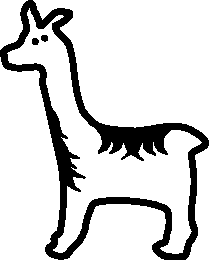
\includegraphics[height=1in]{../graphics/llama.pdf}
\]

\begin{prob}
Take your triangle and denote the measure of its angles as $a$, $b$,
and $c$. We would like to parade Louie around the triangle. There is
only one catch: What happens to Louie when he passes over the ``cut?''
Draw some pictures and see if you can figure it out.
\end{prob}

Start Louie Llama out along a side adjacent to the angle of measure
$a$. He should be on the outside of the triangle, his feet should be
pointing toward the triangle, and his face should be pointing toward
the angle of measure $b$. Continue this process and walk him all
around the triangle. When he gets to the ``cut'' put the paper
together, and let him continue his walk.

\begin{prob} 
Through what angle does Louie rotate when he strolls around a vertex?
\end{prob}

\begin{prob}
How many degrees did the ``cut'' rotate Louie? 
\end{prob}

\begin{prob} 
All in all, how many degrees did Louie Llama rotate in his walk?
\end{prob}


\begin{prob}
If a cone is made on a sheet of paper with a cut of $\theta$ degrees,
and a triangle is made surrounding the point of the cone, what is the
sum of the degrees of this triangle?
\end{prob}




%\begin{prob}
%Explain why not all of Euclid's postulates could hold in this
%universe. Exactly which postulates don't hold?
%\end{prob}
